\subsection{Bibliotecas Android}

\subsubsection{AndroidX}

AndroidX es un conjunto de bibliotecas desarrollada por \textbf{Google} con una serie de herramientas de gran utilidad para el desarrollo en su sistema operativo. Contiene una serie de dependencias que anteriormente formaban parte del paquete \code{android} pero que terminaron por ser extraídas del mismo para ser servidas como bibliotecas opcionales bajo el espacio de nombres \code{androidx}. En este proyecto se han usado varias dependencias de AndroidX:

\begin{itemize}
    \item \textbf{Android KTX}, conjunto de extensiones del lenguaje Kotlin para Android como las corrutinas, utilizadas en el proyecto para la implementación del paralelismo.
    \item \textbf{Appcompat}, proporciona compatibilidad con las nuevas API a versiones anteriores.
    \item \textbf{ConstraintLayout}, otorga un nuevo tipo de layout para las vistas basado en restricciones posicionales. Ha sido el layout más usado en los diseños de las vistas.
    \item \textbf{Lifecycle}. Bibliotecas relacionadas con los ciclos de vida de Android, necesarios en el desarrollo para la programación en paralelo con corrutinas.
    \begin{itemize}
        \item \textbf{Lifecycle KTX}, facilita la programación con ciclos de vida con Kotlin.
        \item \textbf{LiveData KTX}, permite usar los LiveData de Android con las corrutinas de Kotlin.
        \item \textbf{ViewModel KTX}, optimiza la programación con ciclos de vida de los ViewModel de Android en Kotlin. 
    \end{itemize}
    \item \textbf{Navigation}. Bibliotecas para la navegación entre actividades y fragmentos en Android que se utilizó en la aplicación.
    \begin{itemize}
        \item \textbf{Fragment KTX}, navegación en Kotlin para Fragments de Android.
        \item \textbf{UI KTX}, navegación en Kotlin para actividades de Android.
    \end{itemize}
\end{itemize}

Para más información: \href{https://developer.android.com/reference/androidx/packages}{https://developer.android.com/reference/androidx/packages}

\subsubsection{CodeScanner}

Escáner de códigos para Android basado en la librería \textbf{Zxing} (biblioteca también instalada para satisfacer la dependencia) de Google. Proporciona componentes y funciones para crear escáneres de código con diversas características ya implementadas como el enfocado automático, el cambio entre vista de retrato y panorámico o entre las cámaras trasera y delantera. Soporta gran variedad de códigos como matrices de datos o códigos de barra, entre otros. Es un proyecto \emph{open source} creado por \textbf{Yuriy Budiyev} que cuenta con más de una decena de contribuyentes. Fue utilizado en el desarrollo de la aplicación para la implementación del escáner QR.

Para más información: \href{https://github.com/yuriy-budiyev/code-scanner}{https://github.com/yuriy-budiyev/code-scanner}

\subsubsection{Coroutine Test}

Dependencia para pruebas. Proporciona utilidades para la realización eficiente de pruebas con componentes que usen las corrutinas de Kotlin.

Para más información: \href{https://kotlin.github.io/kotlinx.coroutines/kotlinx-coroutines-test/}{https://kotlin.github.io/kotlinx.coroutines/kotlinx-coroutines-test/}

\subsubsection{Espresso}
\label{lib:app:espresso}

Dependencia para pruebas. Espresso es una librería para la realización de pruebas de interfaces de usuario para Android. Ha sido utilizada en las pruebas de integración de la aplicación móvil.

Para más información: \href{https://developer.android.com/training/testing/espresso}{https://developer.android.com/training/testing/espresso}

\subsubsection{JUnit 4}
\label{lib:app:junit4}

Dependencia para pruebas. El framework de desarrollo de pruebas por antonomasia en Java. Como todas las bibliotecas de Java es compatible con Kotlin y ha sido utilizada en el desarrollo para la realización de las pruebas unitarias de la aplicación móvil. Actualmente existe también JUnit 5, que además es complemente retrocompatible con JUnit 3 y JUnit 4. Sin embargo, la experiencia del equipo de desarrollo con dicha biblioteca es menor y por ello se optó por utilizar JUnit 4. Aún con todo, el cambio a JUnit 5 es sencillo y podría hacerse la actualización con facilidad.

Para más información: \href{https://github.com/junit-team/junit4}{https://github.com/junit-team/junit4}

\subsubsection{Material}
\label{lib:app:material}

\begin{wrapfigure}[8]{r}{0.2\textwidth}
    \vspace{-25pt}
    \centering
    
\includegraphics[width=0.2\textwidth]{Implementación/material-icon.png}
    \vspace{-15pt}
    \caption{Logo de Material}
\end{wrapfigure}

Véase \fref{ssec:guia_material_design}. Entre la serie de herramientas que ofrece Material se encuentra una biblioteca de componentes para Android que cumple todas sus guías de estilo. En la aplicación se han seguido las guías de Material para el desarrollo de las interfaces y para facilitar esta tarea se ha utilizado dicha biblioteca para los componentes de las mismas.

Para más información: \href{https://material.io/design}{https://material.io/design}

\subsubsection{Mockk}
\label{lib:app:mockk}

Dependencia para pruebas. Biblioteca de \glspl{mock} para Kotlin, utilidad para la que fue empleada durante el desarrollo en las pruebas unitarias de la aplicación móvil.

Para más información: \href{https://mockk.io/}{https://mockk.io/}

\subsubsection{MockWebServer}
\label{lib:app:mockwebserver}

Dependencia para pruebas. La aplicación hace uso de peticiones a la \acrshort{api} que deben ser simuladas durante la ejecución de las pruebas. Para ello se ha usado MockWebServer, proporcionada por la misma compañía que desarrolla \emph{Retrofit 2} (\ref{lib:app:retrofit2}), que imita la comunicación con un servidor web de forma que se puedan especificar las respuestas a las distintas peticiones y así emular el comportamiento esperado sin necesidad de una comunicación real con la \acrshort{api}.

Para más información: \href{https://github.com/square/okhttp/tree/master/mockwebserver}{https://github.com/square/okhttp/tree/master/mockwebserver}

\subsubsection{NetworkResponseAdapter}

A la hora de realizar comunicaciones por red se deben realizar una serie de comprobaciones y transformaciones de las respuestas recibidas que produce una gran duplicidad del código, lo cual deriva en la necesidad de implementar un sistema de manejo de estas respuestas. Esta biblioteca desarrollada por Kshitij Chauhan con la colaboración de otros usuarios proporciona un adaptador basado en corrutinas que permite la implementación sencilla de código para la conversión y manejo de las respuestas recibidas de estas comunicaciones.

Para más información: \href{https://github.com/haroldadmin/NetworkResponseAdapter}{https://github.com/haroldadmin/NetworkResponseAdapter}.

\subsubsection{Play Services}

\begin{wrapfigure}[4]{r}{0.2\textwidth}
    \vspace{-60pt}
    \centering
    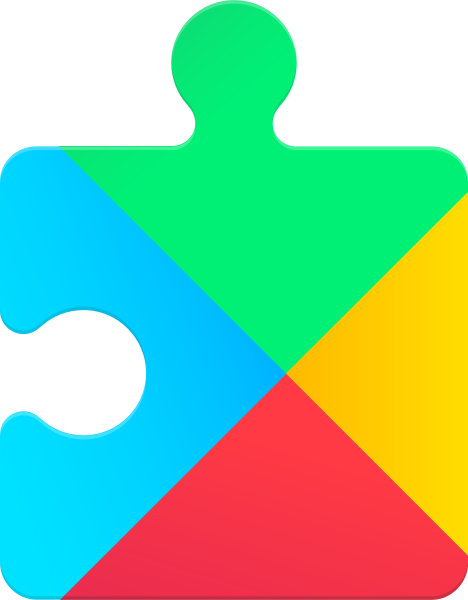
\includegraphics[width=0.15\textwidth]{Implementación/play-services-icon.png}
    \vspace{-15pt}
    \caption{Logo de Play Services}
\end{wrapfigure}

Google ofrece una serie de \acrshort{api}s de desarrollo bajo el espacio de nombres de Play Services. En la aplicaicón han sido utilizadas las siguientes:

\textbf{Auth}
\label{lib:app:auth}

La biblioteca para la implementación de autenticaciones según el flujo de OAuth 2.0\cite{rfc6750} de Google. Ha sido utilizada para implementar con facilidad la lógica de autenticación sin necesidad de verificar las cuentas al poder confianzar en la verificación de Google. Entre otras cosas los componentes permite la validación de las sesiones con un servidor back-end como ha sido el caso en este desarrollo. 

Para más información: \href{https://developers.google.com/identity/sign-in/android/start-integrating}{https://developers.google.com/identity/sign-in/android/start-integrating}

\textbf{Maps for Android}
\label{lib:app:maps}

\begin{wrapfigure}[4]{r}{0.2\textwidth}
    \vspace{-70pt}
    \centering
    
\includegraphics[width=0.15\textwidth]{Implementación/maps-icon.png}
    \vspace{-15pt}
    \caption{Logo de Google Maps}
\end{wrapfigure}

El kit de desarrollo de Maps para Android ha sido utilizado para agregar un mapa de dicho servicio a la aplicación móvil para utilizar en la función de la geolocalización de usuarios.

Para más información: \href{https://developers.google.com/maps/documentation/android-sdk/overview}{https://developers.google.com/maps/documentation/android-sdk/overview}

\textbf{Location}

El último \acrshort{sdk} de PlayServices utilizado en la aplicación va en consonancia con el anterior en el servicio de geolocalización de usuarios. A través de esta \acrshort{api} se obtiene en la aplicación móvil la ubicación espacial del dispositivo que posteriormente se enviará al resto de usuarios asociados.

Para más información: \href{https://developers.google.com/maps/documentation/android-sdk/location}{https://developers.google.com/maps/documentation/android-sdk/location}

\subsubsection{Retrofit 2}
\label{lib:app:retrofit2}

Cliente \acrshort{http} con seguridad de tipos para Android de Square que funciona sobre el OkHttpClient de la misma compañía. Ofrece una \acrshort{api} de muy sencillo manejo que genera toda la lógica para la comunicación con servidores \acrshort{http} a partir de la declaración de interfaces por parte del desarrollador, que únicamente deben especificar el método de la petición, la ruta de misma y el tipo de objeto que será recibido como respuesta. Además, permite la especificación de adaptadores o conversores que gestionen las comunicaciones y generan respuestas que proporcionen directamente una implementación de la clase especificada como tipo de retorno. Ha sido la base de toda la lógica de comunicación con la \acrshort{api} \acrshort{rest}.

Para más información: \href{https://square.github.io/retrofit/}{https://square.github.io/retrofit/}

\subsubsection{Socket.IO}
\label{lib:app:socketio}

Cliente para Android de Socket.IO (véase \fref{lib:api:socket_io}) que permite la especificación y realización de comunicaciones por medio de WebSockets con la WebSocket \acrshort{api}.

Para más información: \href{https://socket.io/blog/native-socket-io-and-android/}{https://socket.io/blog/native-socket-io-and-android/}